%%%%%%%%%%%%%%%%%%%%%%%%%%%%%%%%%%%%%%%%%%%%%%%%%%%%%%%%%%%%%%%%%%%%%%%%%%%%%%%
% Uni Duesseldorf
% Lehrstuhl fuer Datenbanken and Informationssysteme
% Vorlage fuer Bachelor-/Masterarbeiten
% Optimiert fuer den Original-Latex-Kompiler LATEX.EXE (LaTeX=>PS=>PDF)
% Version 1.4 - 2.3.2010
%%%%%%%%%%%%%%%%%%%%%%%%%%%%%%%%%%%%%%%%%%%%%%%%%%%%%%%%%%%%%%%%%%%%%%%%%%%%%%%

%%%%%%%%%%%%%%%%%%%%%%%%%%%%%%%%%%%%%%%%%%%%%%%%%%%%%%%%%%%%%%%%%%%%%%%%%%%%%%%
%%%%%%%%%%% BEGINN EINSTELLUNG FUER DIE ARBEIT. UNBEDINGT ERFORDERLICH! %%%%%%%
%%%%%%%%%%%%%%%%%%%%%%%%%%%%%%%%%%%%%%%%%%%%%%%%%%%%%%%%%%%%%%%%%%%%%%%%%%%%%%%
% Geben Sie Ihren Namen hier an
\newcommand{\bearbeiter}{Alina Elterman}

% Geben Sie hier den Titel Ihrer Arbeit an
\newcommand{\titel}{Game-theoretic Analysis of Strategyproofness in Cake-cutting Protocols}

% Geben Sie das Datum des Beginns and Ende der Bachelorarbeit ein
\newcommand{\beginndatum}{05. September 2011}
\newcommand{\abgabedatum}{05.~Dezember~2011}

% Geben Sie die Namen des Erst- and Zweitgutachters an
\newcommand{\erstgutachter}{Prof. Dr.~J\"org Rothe}
\newcommand{\zweitgutachter}{Prof. Dr.~Peter Kern}

% Falls Sie die Arbeit zweiseitig ausdrucken wollen,
% benutzen Sie die folgende Zeile mit
% \AN fuer zweiseitigen Druck
% \AUS fuer einseitigen Druck
\newcommand{\zweiseitig}{\AUS}

% Falls die Arbeit in englischer Sprache verfasst 
% werden soll, dann benutzen Sie die folgende Zeile mit
% englisch fuer englische Sprache
% deutsch fuer deutsche Sprache
\newcommand{\sprache}{englisch}
%%%%%%%%%%%%%%%%%%%%%%%%%%%%%%%%%%%%%%%%%%%%%%%%%%%%%%%%%%%%%%%%%%%%%%%%%%%%%%%%%
%%%%%%%%%%%%%%%%%%%%%%%%%%%%%%% ENDE EINSTELLUNGEN %%%%%%%%%%%%%%%%%%%%%%%%%%%%%%
%%%%%%%%%%%%%%%%%%%%%%%%%%%%%%%%%%%%%%%%%%%%%%%%%%%%%%%%%%%%%%%%%%%%%%%%%%%%%%%%%

% Die folgende Zeile NICHT EDITIEREN oder loeschen
% (Zum Ab�ndern der BA-Vorlage in eine MA-Vorlage muessen sie
% jedoch die Datei titelmakros1.tex selbst editieren.)
%%%%%%%%%%%%%%%%%%%%%%%%%%%%%%%%%%%%%%%%%%%%%%%%%%%%%%%%%%%
% Obere Titelmakros. Editieren Sie diese Datei nur, wenn
% Sie sich ABSOLUT sicher sind, was Sie da tun!!!
% (Z.B. zum Abaendern der BA-Vorlage in eine MA-Vorlage)
% Uni Duesseldorf
% Lehrstuhl fuer Datenbanken und Informationssysteme
% Version 2.2 - 2.3.2010
%%%%%%%%%%%%%%%%%%%%%%%%%%%%%%%%%%%%%%%%%%%%%%%%%%%%%%%%%%%
\newcommand{\AN}{twoside}
\newcommand{\AUS}{}
%\newcommand{\englisch}{}
%\newcommand{\deutsch}{\usepackage[german]{babel}}

%% Die folgenden auskommentierten Optionen dienen der automatischen
%% Erkennung des Latex-Kompilers und dem Setzen der davon abh�ngigen
%% Einstellungen. Bei Problem z.B. mit dem Einbinden von verschiedenen
%% Grafiktypen bei Verwendung von PdfLatex oder Latex, einfach die
%% verschiedenen \usepackage(s) ausprobieren. (Mit diesen Einstellungen
%% funktionierte diese Vorlage bei der Verwenundg von latex.exe als
%% Kompiler bei den meisten Studierenden.)

%\newif\ifpdf \ifx\pdfoutput\undefined
%\pdffalse % we are not running pdflatex
%\else
%\pdfoutput=1 % we are running pdflatex
%\pdfcompresslevel=9 % compression level for text and image;
%\pdftrue \fi

\documentclass[11pt,a4paper, \zweiseitig]{article}



%\usepackage[iso]{umlaute}
\usepackage[latin1]{inputenc}
\usepackage{palatino} % palatino Schriftart
%\usepackage{makeidx} % um ein Index zu erstellen
\usepackage{tocbibind}
\usepackage[T1]{fontenc} %fuer richtige Trennung bei Umlauten
\usepackage{fancybox} % fuer die Rahmen
\usepackage{shortvrb}
\usepackage{ifthen}
\ifthenelse{\equal{\sprache}{deutsch}}{\usepackage[ngerman]{babel}}{}

\usepackage{lmodern} 
\usepackage{amsmath}
\usepackage{amssymb}
\usepackage{pdfpages}
\usepackage{hyperref}
%\usepackage{fancyheadings}
\usepackage{fancyhdr}
\usepackage{amsfonts}
\usepackage{amsthm}
\usepackage{color}
\usepackage{stmaryrd}
\usepackage{nomencl}
\usepackage[normalem]{ulem} 
\newcommand{\markup}[1]{\uline{#1}}
% Befehl umbenennen in abk
\let\abk\nomenclature

\usepackage{a4wide} % ganze A4 Weite verwenden

%\ifpdf
%\usepackage[pdftex,xdvi]{graphicx}
%\usepackage{thumbpdf} %thumbs fuer Pdf
%\usepackage[pdfstartview=FitV]{hyperref} %anklickbares Inhaltsverzeichnis
%\else
\usepackage[dvips,xdvi]{graphicx}
\usepackage{hyperref} %anklickbares Inhaltsverzeichnis
%\fi

%%%%%%%%%%%%%%%%%%%%%%% Massangaben fuer die Arbeit %%%%%%%%%%%%%%%
\setlength{\textwidth}{15cm}

\setlength{\oddsidemargin}{35mm}
\setlength{\evensidemargin}{25mm}

\addtolength{\oddsidemargin}{-1in}
\addtolength{\evensidemargin}{-1in}

%\makeindex
% Umgebungen f"ur S�tze usw.
\newtheorem*{bemerkung*}{Bemerkung}
\newtheorem*{defi}{Definition}
\newtheorem*{defi*}{Definition}
\newtheorem*{bezeichnungen}{Bezeichnungen}
\newtheorem*{fakt}{Fakt}
\newtheorem*{beispiel}{Beispiel}
\newtheorem*{bsp}{Beispiel}
\newtheorem*{beispiel*}{Beispiel}
\newtheorem*{satz}{Satz}
\newtheorem*{satz*}{Satz}
\newtheorem*{lem}{Lemma}
\newtheorem*{protokoll*}{Protokoll}
\newtheorem*{idee}{Idee}

%definition of new commands
\newcommand{\DGEF}{\text{\textbf{DGEF}}}

\begin{document}

%\setcounter{secnumdepth}{4} %Nummerieren bis in die 4. Ebene
%\setcounter{tocdepth}{4} %Inhaltsverzeichnis bis zur 4. Ebene

\pagestyle{headings}

\sloppy % LaTeX ist dann nicht so streng mit der Silbentrennung
\MakeShortVerb{\�}

\parindent0mm
\parskip0.5em


{
\textwidth170mm 
\oddsidemargin30mm 
\evensidemargin30mm 
\addtolength{\oddsidemargin}{-1in}
\addtolength{\evensidemargin}{-1in}

\parskip0pt plus2pt

% Die Raender muessen eventuell fuer jeden Drucker individuell eingestellt
% werden. Dazu sind die Werte fuer die Abstaende `\oben' und `\links' zu
% aendern, die von mir auf jeweils 0mm eingestellt wurden.

%\newlength{\links} \setlength{\links}{10mm}  % hier abzuaendern
%\addtolength{\oddsidemargin}{\links}
%\addtolength{\evensidemargin}{\links}

\begin{titlepage}
\vspace*{-1.5cm}
  \raisebox{17mm}{
    \begin{minipage}[t]{70mm}
      \begin{center}
        %\selectlanguage{german}
        {\Large INSTITUT F�R INFORMATIK\\}
        {\normalsize
          Lehrstuhl f�r Komplexit\"atstheorie und Kryptologie
\\
        }
        \vspace{3mm}
        {\small Universit�tsstr. 1 \hspace{5ex} D--40225 D�sseldorf\\}
     \end{center}
    \end{minipage}
  }
  \hfill
  
\includegraphics[width=130pt]{bilder/HHU_Logo}
  \vspace{14em}

% Titel
  \begin{center}
      	\baselineskip=55pt
    	\textbf{\huge \titel}
  	 	\baselineskip=0 pt
   \end{center}

  %\vspace{7em}

\vfill

% Autor
  \begin{center}
    \textbf{\Large
      \bearbeiter
    }
  \end{center}

  \vspace{35mm}
 
% Pr�fungsordnungs-Angaben
  \begin{center}
    %\selectlanguage{german}
    
%%%%%%%%%%%%%%%%%%%%%%%%%%%%%%%%%%%%%%%%%%%%%%%%%%%%%%%%%%%%%%%%%%%%%%%%%
% Ja, richtig, hier kann die BA-Vorlage zur MA-Vorlage gemacht werden...
%%%%%%%%%%%%%%%%%%%%%%%%%%%%%%%%%%%%%%%%%%%%%%%%%%%%%%%%%%%%%%%%%%%%%%%%%
    {\Large Bachelorarbeit}

    \vspace{2em}

    \begin{tabular}[t]{ll}
      Beginn der Arbeit:& \beginndatum \\
      Abgabe der Arbeit:& \abgabedatum \\
      Gutachter:         & \erstgutachter \\
                         & \zweitgutachter \\
    \end{tabular}
  \end{center}

\end{titlepage}

}

%%%%%%%%%%%%%%%%%%%%%%%%%%%%%%%%%%%%%%%%%%%%%%%%%%%%%%%%%%%%%%%%%%%%%
\clearpage
\begin{titlepage}
  ~                % eine leere Seite hinter dem Deckblatt
\end{titlepage}
%%%%%%%%%%%%%%%%%%%%%%%%%%%%%%%%%%%%%%%%%%%%%%%%%%%%%%%%%%%%%%%%%%%%%
\clearpage
\begin{titlepage}
\vspace*{\fill}

\section*{Erkl�rung}

%%%%%%%%%%%%%%%%%%%%%%%%%%%%%%%%%%%%%%%%%%%%%%%%%%%%%%%%%%%
% Und hier ebenfalls ggf. BA durch MA ersetzen...
%%%%%%%%%%%%%%%%%%%%%%%%%%%%%%%%%%%%%%%%%%%%%%%%%%%%%%%%%%%

Hiermit versichere ich, dass ich diese Bachelorarbeit
selbstst�ndig verfasst habe. Ich habe dazu keine anderen als die
angegebenen Quellen und Hilfsmittel verwendet.

\vspace{25 mm}

\begin{tabular}{lc}
D�sseldorf, den \abgabedatum \hspace*{2cm} & \underline{\hspace{6cm}}\\
& \bearbeiter
\end{tabular}

\vspace*{\fill}
\end{titlepage}

%%%%%%%%%%%%%%%%%%%%%%%%%%%%%%%%%%%%%%%%%%%%%%%%%%%%%%%%%%%%%%%%%%%%%
% Leerseite bei zweiseitigem Druck
%%%%%%%%%%%%%%%%%%%%%%%%%%%%%%%%%%%%%%%%%%%%%%%%%%%%%%%%%%%%%%%%%%%%%

\ifthenelse{\equal{\zweiseitig}{twoside}}{\clearpage\begin{titlepage}
~\end{titlepage}}{}

%%%%%%%%%%%%%%%%%%%%%%%%%%%%%%%%%%%%%%%%%%%%%%%%%%%%%%%%%%%%%%%%%%%%%
\clearpage
\begin{titlepage}

\section*{\ifthenelse{\equal{\sprache}{deutsch}}{Zusammenfassung}{Abstract}}


%%%%%%%%%%%%%%%%%%%%%%%%%%%%%%%%%%%%%%%%%%%%%%%%%%%%%%%%%%%%%%%%%%%%%%%%%%%%%%%%%
%%%%%%%%%%%%%%%%%%%%%%%%%%%% BEGINN ZUSAMMENFASSUNG %%%%%%%%%%%%%%%%%%%%%%%%%%%%%
%%%%%%%%%%%%%%%%%%%%%%%%%%%%%%%%%%%%%%%%%%%%%%%%%%%%%%%%%%%%%%%%%%%%%%%%%%%%%%%%%
In cake-cutting a protocol instructs the participants how to divide a resource between\\them in a satisfactory manner. A part of those instructions, namely the strategies,\\are optional and can be examined whether they obtain the best solution for the players. If this is not the case, the players have no intention to follow the protocol which can be overruled in this case. Otherwise the protocol is strategyproof.\\Game Theory is designed to determine better strategies. By using a game-theoretic illustration of the cake-cutting problem it is possible to compare all strategies.\\The strategy recommended by the protocol appears to be the best one in the well-known protocols with one exception.  
%%%%%%%%%%%%%%%%%%%%%%%%%%%%%%%%%%%%%%%%%%%%%%%%%%%%%%%%%%%%%%%%%%%%%%%%%%%%%%%%%
%%%%%%%%%%%%%%%%%%%%%%%%%%%%% ENDE ZUSAMMENFASSUNG %%%%%%%%%%%%%%%%%%%%%%%%%%%%%%
%%%%%%%%%%%%%%%%%%%%%%%%%%%%%%%%%%%%%%%%%%%%%%%%%%%%%%%%%%%%%%%%%%%%%%%%%%%%%%%%%

% Die folgende Zeile NICHT EDITIEREN oder loeschen
%%%%%%%%%%%%%%%%%%%%%%%%%%%%%%%%%%%%%%%%%%%%%%%%
% Untere Titelmakros. Editieren Sie diese Datei nur, wenn Sie sich
% ABSOLUT sicher sind, was Sie da tun!!!
%%%%%%%%%%%%%%%%%%%%%%%%%%%%%%%%%%%%%%%%%%%%%%%
\vspace*{\fill}
\end{titlepage}

%%%%%%%%%%%%%%%%%%%%%%%%%%%%%%%%%%%%%%%%%%%%%%%%%%%%%%%%%%%%%%%%%%%%%
% Leerseite bei zweiseitigem Druck
%%%%%%%%%%%%%%%%%%%%%%%%%%%%%%%%%%%%%%%%%%%%%%%%%%%%%%%%%%%%%%%%%%%%%
\ifthenelse{\equal{\zweiseitig}{twoside}}
  {\clearpage\begin{titlepage}~\end{titlepage}}{}
%%%%%%%%%%%%%%%%%%%%%%%%%%%%%%%%%%%%%%%%%%%%%%%%%%%%%%%%%%%%%%%%%%%%%
\clearpage 
\tableofcontents
\thispagestyle{empty}
%\enlargethispage{\baselineskip}
\clearpage \setcounter{page}{1}
%%%%%%%%%%%%%%%%%%%%%%%%%%%%%%%%%%%%%%%%%%%%%%%%%%%%%%%%%%%%%%%%%%%%%
% Leere Seite, falls Inhaltsverzeichnis mit ungerader Seitenzahl und 
% doppelseitiger Druck
%%%%%%%%%%%%%%%%%%%%%%%%%%%%%%%%%%%%%%%%%%%%%%%%%%%%%%%%%%%%%%%%%%%%%
\ifthenelse{ \( \equal{\zweiseitig}{twoside} \and \not \isodd{\value{page}} \)}
	{\pagebreak \thispagestyle{empty} \cleardoublepage}{\clearpage}



%%%%%%%%%%%%%%%%%%%%%%%%%%%%%%%%%%%%%%%%%%%%%%%%%%%%%%%%%%%%%%%%%%%%%
%%%%%%%%%%%%%%%%%%%%%%%%% BEGINN TEXTTEIL %%%%%%%%%%%%%%%%%%%%%%%%%%%
%%%%%%%%%%%%%%%%%%%%%%%%%%%%%%%%%%%%%%%%%%%%%%%%%%%%%%%%%%%%%%%%%%%%%
\section{Introduction}
It is Christmas party in the cakes4people agency. Everybody is waiting expectantly on the big promised cake at the end of the party. This cake has been spectacular in the past years. A lot of different cake layers, different fruits on top and even chocolate sprinkles over parts of the cake have been so delicious. So it's no wonder that everyone wants to get as much as possible of this culinary treat, and especially of their individual favourite part. Nevertheless, the people like their colleagues and want still to be as fair as possible to them.\\A new employee is also celebrating with the group. Rumors have been told a lot about him, but no one has managed to assess him or his preferences properly. Nevertheless, he also takes part in the big cake division. He even wants to change the allocation procedure. He promises that everyone can keep their wishes private, each of them just needs to make a couple of simple decisions and will get their best possible share.\\But the people become suspicious. Different questions occur in their minds: ''What if he has a strategy he is not telling us about, which promises him a better piece? What if he is lying about his preferences? Why should we trust him?''
The chief sees the mistrust and knows how to reassure the people. He is a game theory enthusiast and promises to show them that the proposed procedure is strategyproof. Hereby, only by taking actions truthful a participant can always get his best possible piece.\\
Strategyproofness of an allocation procedure ...
\begin{comment}
%Erklären was ist FAIR DIVISION\\ Kuchen geschnitten, nicht geteilt Krimi
%%A desirable property for cake-cutting protocols is strategy-proofness [6]. A protocol is strategy-proof if there is no incentive for any player to lie about his utility function. A protocol defines what to do for each player pi according to its utility function i. Since i is unknown to any other player, pi can execute some action that differs from the protocol’s definition (by pretending that pi ’s utility function is  ′i(≠ i)). If pi obtains more utility by lying about his utility function, the protocol is not strategy-proof. If a protocol is not strategy-proof,each player has to consider what to do and the result might differ from the intended result. If a protocol is strategy-proof, the best policy for each player is simply observing the rule of the protocol.%%
%(kein sehr guter anfang gez. herr rothe)Strategic play, cheating, incentive compatible, risk aversion, truthfulness, strategyproof and a lot more. All of them are keywords of whether an algorithm can resist the actions of selfish players and their greediness.
%Cake-cutting is part of interdisciplinary fields like economics, mathematics, operations research, political and computer science. Game theory is fulfilling the same property. Except for this fact, they have hardly something in common. While cake cutting is about fair division of a heterogeneous divisible good, where the studies are especially concentrated on types of fairness, game theory studies the strategies people use when making decisions.\\
%The role of strategies has not been widely researched yet in the context of cake cutting. But their importance is indisputable, with respect to fairness. Imagine the following situation:
%Example Cost Sharing from Algorithmic GT Noam Nissan chap. 15
%\begin{itemize}
%\item{division of sports tickets, health resources, computer networking resources, voting power, intellectual property licenses, costs for environmental improvements, etc}
%\item{formalize fairness, including max-min fairness, proportional fairness, envy-free fairness, etc. which may or may not lead to stable allocations in the sense of say Nash Equilibrium, or strong Nash Equilibrium}
%\end{itemize}
%Es werden Auswirkungen von nicht ehrlichen Strategien auf die Gerechtigkeit von Protokollen betrachtet. Der approach der Neidfreiheit ist zu stark, da kein finite bounded Protokoll f"ur n >3 (>4 f"ur allgemein) bekannt ist. Dagegen w"are der approach der Proportionaltit"at zu schwach, $\dots$. Das notwendige Mittelmaß liefert der DGEF und so fällt der Focus dieser Arbeit auf die Möglichkeit den DGEF eines Protokolles durch unehrliche Strategien zu erhöhen. Die Analyse erfolgt mittels Spieltheorie.\\
%\newline
%$\cdot$ Able to show that the only strategy promising a fair share is the recommended one.
\end{comment}
\pagebreak
%%%%%%%%%%%%%%%%%%%%%%%%%%%%%%%%%%%%%%%%%%%%%%%%%%%%%%%%%%%%%%%%%%%%%%%%%%%%%%%%%%%%%%%%%%%%%%%%%%%%%%%%%%%%%%%%
%%%%%%%%%%%%%%%%%%%%%%%%%%%%%%%%%%%%%%%%%%%%%%%%%%%%%%%%%%%%%%%%%%%%%%%%%%%%%%%%%%%%%%%%%%%%%%%%%%%%%%%%%%%%%%%%
%%%%%%%%%%%%%%%%%%%%%%%%%%%%%%%%%%%%%%%%%%%%%%%%%%%%%%%%%%%%%%%%%%%%%%%%%%%%%%%%%%%%%%%%%%%%%%%%%%%%%%%%%%%%%%%%
\subsection{Related Work}
Recently, two papers, \cite{chen:truth} and \cite{tamuz}, with the focus on strategyproofness have been published. In \cite{chen:truth} they weakened the assumptions of cake cutting by including the free disposal assumption, which can lead to a not complete allocation of the cake and allow only piecewise uniform valuations. The second restriction is indeed very hard. Their goal was to give a proportional, envy-free, polynomial and strong strategyproof protocol. In \cite{tamuz} the authors invented new procedures including a referee, who has full knowledge. This extension is a restriction of cake-cutting as well. Both papers also researched truthfulness in expectation for protocols with randomness.\\ \newline
In pie-cutting \cite{why} showed that a strategyproof and efficient mechanism must be dictatorial. The definition of strategyproofness in this paper is a much stronger condition. Also pie-cutting slightly differs from cake-cutting, since the pie ist represented as a circular object and the cuts are wedges. The results for pie-  and cake-cutting do not carry over to each other, but the definition of strategyproofness does. \cite{pie} gave more details in the context of pie-cutting and strategyproofness. \\
\newline
The start of reaserching strategyproofness was \cite{brams}, where the authors introduced a fitting definition of strategyproofness and proved that two procedures called SP and EP are strategyproof.\\ A response on their work was a counterexample by \cite{ccc}. After admitting their mistake, in \cite{note} they restricted their first definition to cases with non-equal valuation functions and introduced a new general definition for strategyproof cake-cutting.\\
In \cite{dc} and in the revisited version of this work \cite{dc2} the authors focused on the Divide-and-Conquer protocol and showed that it is strategyproof for risk averse players. In the later work they call this property truth-inducing. \\ \cite{lindner:degrees} parallelyzed the Last-Diminisher and proved that this new protocol is also strategyproof for risk-averse players. \pagebreak
%%%%%%%%%%%%%%%%%%%%%%%%%%%%%%%%%%%%%%%%%%%%%%%%%%%%%%%%%%%%%%%%%%%%%%%%%%%%%%%%%%%%%%%%%%%%%%%%%%%%%%%%%%%%%%%%
%%%%%%%%%%%%%%%%%%%%%%%%%%%%%%%%%%%%%%%%%%%%%%%%%%%%%%%%%%%%%%%%%%%%%%%%%%%%%%%%%%%%%%%%%%%%%%%%%%%%%%%%%%%%%%%%
%%%%%%%%%%%%%%%%%%%%%%%%%%%%%%%%%%%%%%%%%%%%%%%%%%%%%%%%%%%%%%%%%%%%%%%%%%%%%%%%%%%%%%%%%%%%%%%%%%%%%%%%%%%%%%%%
\section{Preliminaries}
\subsection{Basics of Cake-cutting}
It is necessary to define the components and challenges of cake-cutting. But first, what exactly is cake-cutting about? It involves a set of $n \in \mathbb{N}$ players $P_n=\{p_1,\ldots,p_n\}$. It is assumed that each of them wants to get as much as possible of the divided resource. The goal is to find an allocation of a single, divisible and heterogeneous good between the $n$ players.  
	\begin{figure}[h]
		\centering
 		 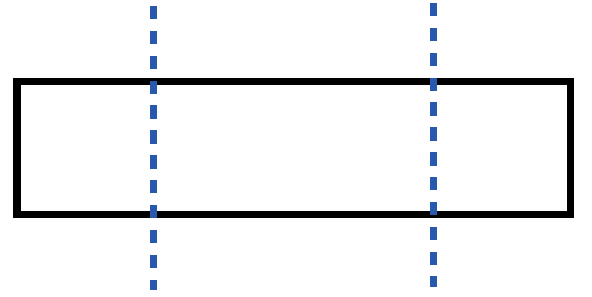
\includegraphics[width=120pt]{kek.pdf}
   \caption{Cake}Example for a visualisation of a cake with two cuts
  	 \end{figure} 
Such an allocation has to be of a special kind, so that the involved players are pleased with the outcome. For the visualization it is common to use a rectangular cake. The division is performed by parallel cuts. The cake $X$ is represented by the unit interval $X=[0,1] \subseteq \mathbb{R}$. Each subinterval $X'\subseteq X$ or a sequence of disjoint subintervals $$\sideset{}{ }\bigcup\limits_{m\in\mathbb{N}}X'_m$$
with $X'_m\subseteq X$ is called a \emph{portion (or piece)}. The portion of the cake which is received by player $p_i$ is denoted $X_i$. The state is called an \emph{allocation}, when all portions of the cake are owned by players. Each piece has a public size, which can be computed as the sum of all border differences, and the private value of each player, which is constituted by the lower defined valuation function.\\

Every player $p_i\in P_n$ has a \emph{valuation function (valuation)} $v_i:\{X'|X' \subseteq X\} \rightarrow [0,1]$ with the following properties:
\begin{enumerate}
\item Non-negativity: $v_i(C)\geq 0$ for all $C\subseteq X.$
\item Normalisation: $v_i(\emptyset)=0$ and $v_i([0,1])=1.$
\item Additivity: $v_i(C \cup C')=v_i(C)+v_i(C')$ for disjoint
$C,C'\subseteq X.$\footnote{Monotonicity: If $C' \subseteq C$ then $v_i(C') \leq v_i(C)$. Monotonicity follows from additivity, because for the assumption $C' \subseteq C$ and $A:=C\backslash C'$: $v_i(C)=v_i(A\cup C')=v_i(A)+v_i(C')=\underbrace{v_i(C\backslash C')}_{\geq 0}+v_i(C')\geq v_i(C').$}
\item Divisibility: For all $C\subseteq [0,1]$ and all $\alpha \in
\mathbb{R}$, $0\leq \alpha \leq 1$, there exists a $B\subseteq C$, so that
$v_i(B)=\alpha \cdot v_i(C).$
\item  $v_i$ is continuous: If $0<x<y\leq 1$ with $v_i([0,x])=\alpha$ and
$v_i([0,y])=\beta$, then for every $\gamma \in [\alpha,\beta]$ there exists a $z \in [x,y]$ so that $v_i([0,z])=\gamma.$
\item Non-atomic:  $v_i([x,x])=0$ for all $x\in X.$
\end{enumerate}
%Game theory can be seen as a tool for describing interaction in life's processes. The occurring problems can be simulated by games.  
%Non-cooperated game theory is about single selfish players, and in cooperated the main focus is on forming coalitions. For computer scientists especially the algorithmic game theory is of major interest, because $\dots$. 
\subsection{Concepts in Game Theory}
Basic concepts from game theory are described and directly applied to the cake-cutting problem. %The comparison between the classes of games indicate that the best fitting game-theoretic model is the Bayesian game \cite{}. The development of this result and use of the associated solution concepts is described.
In particular the priority have the possible representations of games. For further reading see \cite{}, \cite{} and \cite{ba}. 
\begin{defi}{\textbf{(Game)}}\\
\emph{A \emph{non-cooperative game} $\Gamma=(P_n,S,u)$ consists of the set of players $P_n$, the set of strategies $S$ and the set of utility functions (pay-off) of all players $u$.
\begin{itemize}
\item Each player in the set $P_n=\{p_1,\cdots,p_n\}$ behaves selfish and rational.
\item Each player has his own set of strategies. A \emph{pure strategy} is a single action. A \emph{mixed strategy} is a probability distribution over pure strategies.
\item Utility is a real-valued quantity measuring an player's happiness. A utility function is a mapping from outcomes to utilities. The agent is indifferent between outcomes with equal utilities and strictly prefers outcomes with higher utilities.
\end{itemize}}
\end{defi}
Each game has also an end-state, which is usually called outcome. In cake-cutting an outcome is an allocation.
%Definition 2 (Outcome) An outcome is any end-state of the system.
The utility function in cake-cutting is the valuation function. The utility of an allocation for a player is the value of the piece this player obtain in it.
\begin{defi}{\textbf{(Strategies)}}\\
\emph{ Assume two strategies $S_1$ and $S_2$ for a player $p_1$ and the value $v_1(X_{1,S_1,i})$ and $v_1(X_{1,S_2,i})$ for $i \in \mathbb{N}$ number of possible different allocations.\\
	The strategy $S_1$ \emph{dominates} the strategy $S_2$ if $v_1(X_{1,S_1,i}) \geq v_1(X_{1,S_2,i})$ for all $i$.
		\begin{itemize}
			\item The strategy $S_1$ \emph{strictly dominates} the strategy $S_2$ if $v_1(X_{1,S_1,i}) > v_1(X_{1,S_2,i})$ for all $i$.
			\item The strategy $S_1$ \emph{weakly dominates} the strategy $S_2$ if $v_1(X_{1,S_1,i}) > v_1(X_{1,S_2,i})$ for at least one $i$ and $v_1(X_{1,S_1,i}) \geq v_1(X_{1,S_2,i})$ for all other $i$.
		\end{itemize}
	}\emph{
}\emph{
The strategy $S_1$ is \emph{dominated} by the strategy $S_2$ if $v_1(X_{1,S_1,i}) \leq v_1(X_{1,S_2,i})$ for all $i$.
\begin{itemize}
\item The strategy $S_1$ is \emph{strictly dominated} by the strategy $S_2$ if $v_1(X_{1,S_1,i}) < v_1(X_{1,S_2,i})$ for all $i$.
\item The strategy $S_1$ is \emph{weakly dominated} by the strategy $S_2$ if $v_1(X_{1,S_1,i}) < v_1(X_{1,S_2,i})$ for at least one $i$ and $v_1(X_{1,S_1,i}) \leq v_1(X_{1,S_2,i})$ for all other $i$.
\end{itemize}}
\end{defi}
The strategy $S_1$ can be neither dominates nor dominated regarding an other strategy $S_2$, so $v_1(X_{1,S_1,i}) < v_1(X_{1,S_2,i})$ for at least one $i$ and $v_1(X_{1,S_1,i}) > v_1(X_{1,S_2,i})$ for all other $i$. Also  $v_1(X_{1,S_1,i}) = v_1(X_{1,S_2,i})$ for all $i$ is possible, but in this case the strategies can be seen as equal and the player is indifferent between them.\\
A game can be rather strategic, where all player move simoultaneous or extensive, where the players move in a fixed or variable order.
%\begin{defi}{\textbf{(Zero-Sum Game / General-Sum Game )}}\\
%\emph{In a \emph{zero-sum game} the sum of the valuations of an allocation is one. Otherwise the game is called %\emph{variable-sum game}.}
%\end{defi}
%Cutting a cake is usually a non-zero-sum game since it allows players to get better off than $\nicefrac{1}{n}$-th. An exception is a cake with equal valuations over the cake.
%\begin{defi}{\textbf{(Repeated Game)}}\\
%\emph{A \emph{repeated game} } 
%\end{defi}
\newline
\newline
\textbf{Information in Games}
\begin{defi}{\textbf{(Perfect / Imperfect Information)}}\\
Perfect information extensive form games are games in tree representation where every inner node represents
a choice by a single agent, with the out-edges of the node being the possible actions.
Each leaf node is an outcome labeled by a vector of utilities (one per agent).
\end{defi}
\begin{defi}{\textbf{(Complete / Incomplete Information)}}\\
An imperfect information extensive form games are extensive form games where the agent cannot distinguish
two or more choice nodes (those nodes are said to belong to an equivalence set).
\end{defi}
\begin{comment}
(Pure strategy (extensive form game)) pure strategy for an extensive form game is a mapping from nodes or equivalence sets to actions {analogous
to a policy in decision theory.)\\

(Induced normal form (extensive form game)) We can convert an extensive form game into a normal form game (called the "induced normal form ") where
the normal form game's actions are pure strategies in the extensive form game. The payoffs in the normal form game are taken front the leaf-node reached by following
those strategies. Because every extensive form game has a corresponding induced normal form
game, it must have a Nash equilibrium (by Theorem 27).
\end{comment}
\begin{defi}{\textbf{(Bayesian Game)}}\\
A Bayesian Game is a set of players, each of which has a set of actions and a utility function mapping action and type profiles to utility. A Bayesian game also includes a distribution over type profiles.
\end{defi}

Often, strategic interactions involve some notion of random events and private information. We model these using Bayesian games. Many card games (for example, poker) are instances of this type of interaction.\\

Definition 39 (Type) An agent's type is a complete representation of his private information.\\
Definition 40 (Type profile) A type profile is a vector of types, one per agent. One simple but powerful way to represent Bayesian games is to say that the agents have different information about which normal form game they are actually playing.
\begin{comment}
Definition 43 (Pure strategy (Bayesian game)) A pure strategy in a Bayesian game
is a function mapping from type to action.
An alternative way of representing Bayesian games is to model them as extensive
form games where one of the agents is actually a random process (with all the real
agents having full common knowledge of the probabilities):\\
Definition 44 (Bayesian game (extensive form representation)) The extensive form
representation of a Bayesian game augments a conventional imperfect information ex-
tensive form game with "chance nodes" where each branch is chosen according to
some (commonly known) probability.
Extensive form representations of Bayesian games have the same pure strategy
space as regular extensive form games.\\
Definition 46 (Induced normal form (Bayesian game)) The induced normal form of
a Bayesian game is a normal form game where each action is a pure strategy in the
Bayesian game. The values in the cells of the table are filed in by computing the ex
ante expected utility of each pure strategy prof le.
When discussing the properties of Bayesian games, the amount of information
available must be defined (particularly when taking expectations). We characterize
this by the terms ex ante, ex interim and ex post.
Definition 47 (Ex ante) Ex ante refers to situations where no agent's type is fixed or
known.
Definition 48 (Ex interim) Ex interim refers to situations where exactly one agent's
type is known.
Definition 49 (Expost) Ex ante refers to situations where all agent's types are known.\\
\newline
\end{comment}
For issues in cutting a cake it is especially important that the valuation functions are private and that no player knows each others type or his own position in the game. So for the analysis some assumption have to be made and a stochastic model to be defined.
\begin{defi}{\textbf{(Probability Model)}}\\
\emph{The sample space $S$ of a random phenomenon is the set of all possible outcomes. An event is an outcome or a set of outcomes of a random phenomenon. That is, an event is a subset of the sample space. A \emph{probability model} is a mathematical description of a random phenomenon consisting of two parts: a sample space $S$ and a way of assigning probabilities to events.} 
\end{defi}
\begin{defi}{\textbf{(Expected Value)}}\\
A 
\end{defi}
A game can be represented in normal or in extended form. The normal form is advantageous for games where players move simultaneous, which is not often the case in cake-cutting. So rather the presentation in extended form as a game tree will be used in this work.
\begin{defi}\textbf({Normal Form Game)}\\
\emph{A \emph{normal form game} is a tabular representation of a game. In the case for two players the first player chases the row while the second choses the column. Each cell contains a vector with the value of the obtained piece, one per player.}
\end{defi}
\begin{table}[htb]
\centering
 \renewcommand{\arraystretch}{1.2} 
\begin{tabular}{c|c|c|}
\cline{2-3}
&\multicolumn{1}{|c|}{$Strategy_a$}& {$Strategy_b$}\\
\hline
\multicolumn{1}{|r|}{$Strategy_I$}&$\left(v_1(X_{1,I,a}), v_2(X_{2,I,a}) \right)$&$\left(v_1(X_{1,I,b}), v_2(X_{2,I,b}) \right)$\\
\hline
\multicolumn{1}{|r|}{$Strategy_{II}$}&$\left(v_1(X_{1,II,a}), v_2(X_{2,II,a}) \right)$&$\left(v_1(X_{1,II,b}), v_2(X_{2,II,b}) \right)$\\
\hline
\end{tabular}
\caption{Game in normal form}\label{Table0}
\end{table}
\begin{defi}\textbf({Extended Form Game)}\\
\emph{An \emph{extended form game} is a tree representation of a game. In the case for two players the first player ...}
\end{defi}
\begin{figure}[h!]
\begin{center}
	\begin{tikzpicture}
		\node[circle,draw,ball color=blue!10,shade=ball,inner sep=5pt] (n1) at (1,5) { };
		\node[circle,draw,ball color=blue!10,shade=ball,inner sep=5pt] (n2) at (5,7) {};
		\node[circle,draw,ball color=blue!10,shade=ball,inner sep=5pt] (n3) at (5,3) {};
		\node[circle,draw,ball color=blue!10,shade=ball,inner sep=5pt] (n4) at (9,8) {};
		\node[circle,draw,ball color=blue!10,shade=ball,inner sep=5pt] (n5) at (9,6) {};
		\node[circle,draw,ball color=blue!10,shade=ball,inner sep=5pt] (n6) at (9,4) {};
		\node[circle,draw,ball color=blue!10,shade=ball,inner sep=5pt] (n7) at (9,2) {};

		\node[draw=none,fill=none] (t1) at (1,5.5) {1};
		\node[draw=none,fill=none] (t2) at (5,7.5) {2};
		\node[draw=none,fill=none] (t1) at (5,3.5) {2};

		\node[draw=none,fill=none,right] at (1.85,6.55) {$Strategy_{I}$};		
		\node[draw=none,fill=none,right] at (1.85,3.5) {$Strategy_{II}$};
		\node[draw=none,fill=none,right] at (6,2.2) {$Strategy_{b}$};
		\node[draw=none,fill=none,right] at (6,3.9) {$Strategy_{a}$};
		\node[draw=none,fill=none,right] at (6,6.2) {$Strategy_{b}$};
		\node[draw=none,fill=none,right] at (6,7.9) {$Strategy_{a}$};
		\node[draw=none,fill=none,right] at (9.5,8) {$\left(v_1(X_{1,I,a}), v_2(X_{2,I,a})\right)$};
		\node[draw=none,fill=none,right] at (9.5,6) {$\left(v_1(X_{1,I,b}), v_2(X_{2,I,b})\right)$};
		\node[draw=none,fill=none,right] at (9.5,4) {$\left(v_1(X_{1,II,a}), v_2(X_{2,II,a}) \right)$};
		\node[draw=none,fill=none,right] at (9.5,2) {$\left(v_1(X_{1,II,b}), v_2(X_{2,II,b}) \right)$};

		\draw (n1) -- (n2);
		\draw (n1) -- (n3);
		\draw (n2) -- (n4);
		\draw (n2) -- (n5);
		\draw (n3) -- (n6);
		\draw (n3) -- (n7);

	\end{tikzpicture}
	\caption{Game in extended form}
\end{center}
\end{figure}
%%%%%%%%%%%%%%%%%%%%%%%%%%%%%%%%%%%%%%%%%%%%%%%%%%%%%%%%%%%%%%%%%%%%%%%%%%%%%%%%%%%%%%%%%%%%%%%%%%%%%%%%%%%%%%%%
%%%%%%%%%%%%%%%%%%%%%%%%%%%%%%%%%%%%%%%%%%%%%%%%%%%%%%%%%%%%%%%%%%%%%%%%%%%%%%%%%%%%%%%%%%%%%%%%%%%%%%%%%%%%%%%%
%%%%%%%%%%%%%%%%%%%%%%%%%%%%%%%%%%%%%%%%%%%%%%%%%%%%%%%%%%%%%%%%%%%%%%%%%%%%%%%%%%%%%%%%%%%%%%%%%%%%%%%%%%%%%%%%
%%%%%%%%%%%%%%%%%%%%%%%%%%%%%%%%%%%%%%%%%%%%%%%%%%%%%%%%%%%%%%%%%%%%%%%%%%%%%%%%%%%%%%%%%%%%%%%%%%%%%%%%%%%%%%%%
%%%%%%%%%%%%%%%%%%%%%%%%%%%%%%%%%%%%%%%%%%%%%%%%%%%%%%%%%%%%%%%%%%%%%%%%%%%%%%%%%%%%%%%%%%%%%%%%%%%%%%%%%%%%%%%%
%%%%%%%%%%%%%%%%%%%%%%%%%%%%%%%%%%%%%%%%%%%%%%%%%%%%%%%%%%%%%%%%%%%%%%%%%%%%%%%%%%%%%%%%%%%%%%%%%%%%%%%%%%%%%%%%
%%%%%%%%%%%%%%%%%%%%%%%%%%%%%%%%%%%%%%%%%%%%%%%%%%%%%%%%%%%%%%%%%%%%%%%%%%
%%%%%%%%%%%%%%%%%%%%%%%%%%%%%%% ENDE TEXTTEIL %%%%%%%%%%%%%%%%%%%%%%%%%%%%
%%%%%%%%%%%%%%%%%%%%%%%%%%%%%%%%%%%%%%%%%%%%%%%%%%%%%%%%%%%%%%%%%%%%%%%%%%

\clearpage
\bibliography{references.bib}
\bibliographystyle{apalike}
\thispagestyle{empty}
%\vspace*{\fill}g
\pagestyle{plain}
\clearpage

\listoffigures

\listoftables
\thispagestyle{empty}
%\pagebreak
\pagestyle{plain}
%\printindex
\end{document}